\section{Visualization}
\label{sec:prototype-semantics:visualization}
We use \DOT, which is described in Appendix~\ref{ap:tools}, to visualize the state spaces of \SLCO models by translating \LTS representations to graphs in the format of the \DOT language.
State spaces represented in \LTS are transformed to \DOT graphs by translating all states to nodes and all transitions to edges, and specifying how initial states, final states, and normal states should be visualized.

\begin{figure}[hbt]
  \centering
  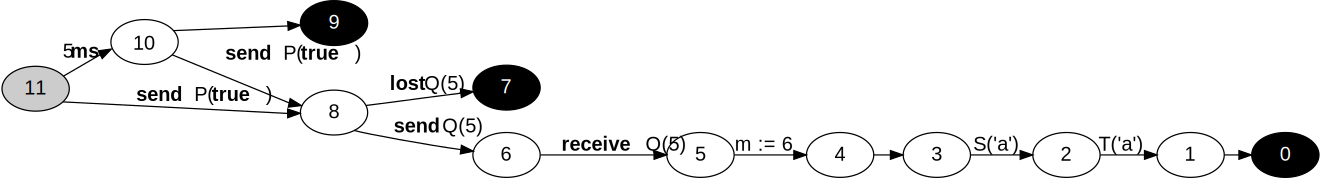
\includegraphics[scale=.36]{prototype-semantics/figs/statespace-orig}
  \caption{A state space visualized using \DOT}
  \label{fig:prototype-semantics:statespace}
\end{figure}

Figure~\ref{fig:prototype-semantics:statespace} shows the labeled transition system that represents the state space of the model in Figure~\ref{fig:slco:SLCOExampleCommunication}, \ref{fig:slco:SLCOExampleStructure}, and~\ref{fig:slco:SLCOExampleSMSMinimized}, visualized using \DOT.
In the visual representation, the transition labels are placed above the corresponding transition.
The unlabeled transitions in the state space of Figure~\ref{fig:prototype-semantics:statespace} correspond to transitions with expressions in the \SLCO model whose behavior is described by the state space.

\begin{figure}[hbt]
  \centering
  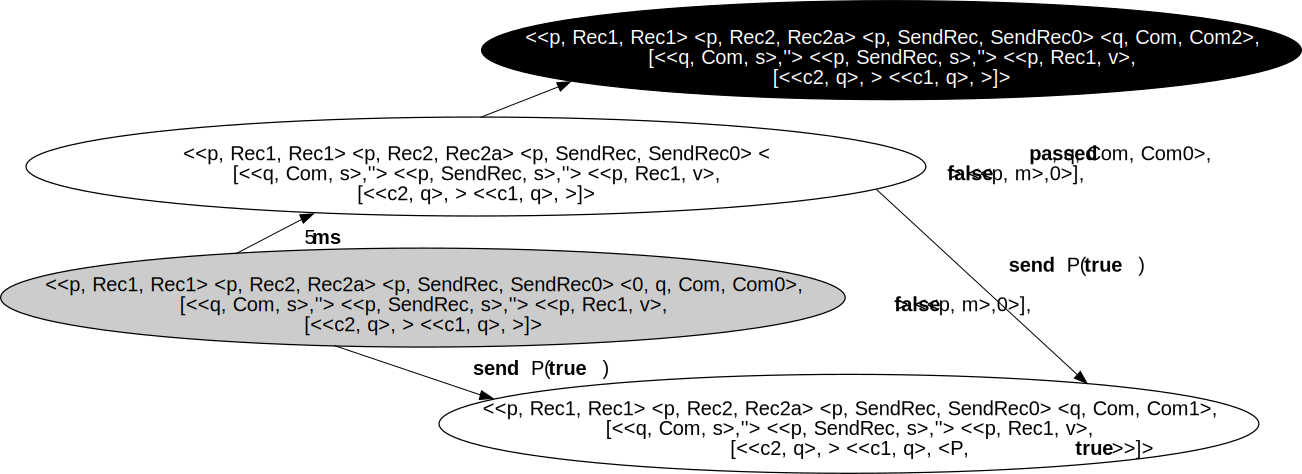
\includegraphics[scale=.36]{prototype-semantics/figs/debug}
  \caption{A more detailed visualization for debugging}
  \label{fig:prototype-semantics:debug-statespace}
\end{figure}

\CS representations of configurations and steps, such as the ones in Listings~\ref{lst:prototype-semantics:steps} and~\ref{lst:prototype-semantics:time_steps}, list all reachable configurations and steps for a given \SLCO model.
Therefore, design decisions can be evaluated by inspecting the \CS representations of a number of models while developing the executable prototype of the semantics of \SLCO.
However, visual representations of the same information, such as the state space in Figure~\ref{fig:prototype-semantics:statespace}, provide a more convenient way of checking whether the semantics implemented by means of the various transformation tools coincides with the intended semantics.
Using the visual representation, it is often easier to spot unintended behavior.

Once unintended behavior is encountered, more information about the configurations can help to locate and repair the parts of the tools that cause this behavior.
The desire for more detailed information lead to the implementation of the tool~\CStoDot, which translates \CS representations directly to more elaborate \DOT graphs.
In Figure~\ref{fig:prototype-semantics:debug-statespace}, the four leftmost states of the state space in Figure~\ref{fig:prototype-semantics:statespace} are shown in this elaborate graphical representation, along with a number of the related transitions.

\begin{figure}[hbt]
  \centering
  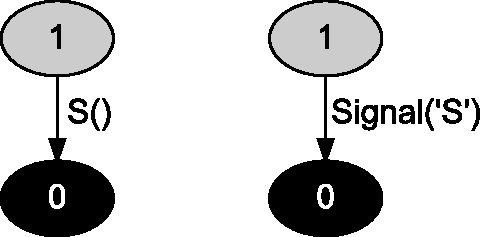
\includegraphics[scale=.36]{prototype-semantics/figs/transformation-comparison}
  \caption{State spaces before and after refinement}
  \label{fig:prototype-semantics:compare-statespace}
\end{figure}

The various textual and graphical representations of the behavior of \SLCO models described above have also been used during the development of model transformations.
By generating the state space of both the source and target model for a given transformation and comparing these state spaces, the effect of the transformation can be studied.
For instance, Figure~\ref{fig:prototype-semantics:compare-statespace} shows the state space of a small \SLCO model before and after applying transformation~\Transformation{arg}, which is described in Section~\ref{subsubsec:slco:endogenous:arg}.
The figure clearly shows that the transformation has no unwanted side effects.
Because of its complexity, we used this approach to develop transformation~\TGen described in Section~\ref{subsubsec:slco:sync2async}.